\section{Analysis}
\label{sec:sec002}

To improve possibilities for PAM, I emphasize the need for collaborative work to develop standardized methods and analysis regarding the independent monitoring of the livestock production domain.
This section is addressing a descriptive analysis of the potential for a novel robust theoretical and analytical framework for monitoring vocalizing livestock productions.
The current applications of PAM technologies, identify challenges and research priorities at each stage of the PAM pipeline (Figure \ref{fig:img002}), as well as significant emerging trends for PAM in research.

The workflow (Figure \ref{fig:img002}) is presented as (a) commercial acoustic sensors (\textit{AudioMoth}) installation; (b) comparison of audio data collected using different sensor models and sampling protocols; (c) recording and storing audio; (d) processing sound files and metadata; (e) sound identification pipeline for spatially and temporally explicit record of animal call detections; (f) statistical analysis of animal data; and (g) finding patterns of animal acoustic indicators.

%%%%%%%%%%%%%%%%%%%%%%%%%%%%%%%%%%%%%%%%%%%%%%%%%%

\hfill

\begin{figure}[!ht]
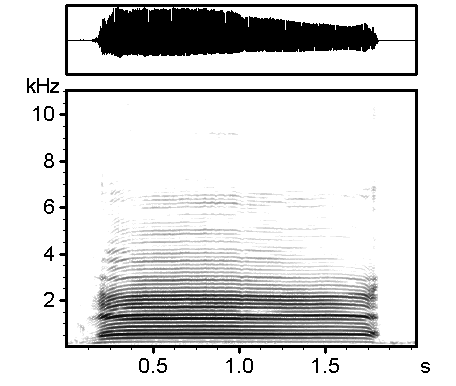
\includegraphics[width=\columnwidth]{img006}
\caption{Sheep sound recording sample (avisoft.com/sounds.htm)~\cite{astuti2011animal}. A description of externally recorded sample in different poses. From this image we can have an idea of how is the behavior of sheep vocalization and what to expect.}
\label{fig:img006}
\end{figure}

\hfill

%%%%%%%%%%%%%%%%%%%%%%%%%%%%%%%%%%%%%%%%%%%%%%%%%%

Commercial acoustic sensors (Figure \ref{fig:img002}.a) are now comparable to image processing in terms of user-accessibility and durability~\cite{gibb2018emerging}.
The programmable schedules and onboard metadata collection, allow for extended autonomous deployments with flexible sampling regimes within improved battery life and storage.
On the other hand, costs have limited scalability, with ubiquitous models in comparison to the image acquisition hardware.

By using different sensor models and sampling protocols, we can achieve a higher understanding of the comparability for audio data collected.
The use of different sensor models and sampling protocols across different environments is also an ongoing challenge (Figure \ref{fig:img002}.b).
PAM studies commonly deploy static sensors (analogous to image processing) either standalone, in multi-sensor networks, or in linked arrays to allow for sound localization.
In particular cases, the use of these components ({\em e.g.}, microphones) might involve tradeoffs between sensor data quality and cost.
For instance, if showing inconsistent frequency response, vulnerable to environmental damage, or lower signal-to-noise ratios.
A critical question concerns how much data can be a sacrifice without comprising the capacity to derive sufficient information from audio.
The answer may vary taxonomically since each specific individual animal is intrinsically hard to distinguish between others.

\break

Recording and storing audio at sufficient quality (Figure \ref{fig:img002}.c) is therefore crucial, alongside with detailed metadata.
Both recording parameters and sensor type are also providing opportunities to address additional questions.
Another possible solution, to data capacity issues, could be reducing the stored amount of audio.
For instance, by applying algorithms that only trigger recording when monitorization is needed or applying onboard thresholds.
However, discarding audio data is undesirable.
Still, some degree of prior filtering can prevent datasets becoming large, as well as if we combine it with wireless data transmission, we could facilitate real-time livestock monitoring and reporting across animal productions.

The complexity of environmental audio ({\em e.g.}, communication between animal individuals, localization or vocal health issues) offers a useful real-world test for new methods (Figure \ref{fig:img002}.d).
The involvement of the Machine Learning (ML) and Computer Vision (CV) in PAM is driving analytical advantages benefitting the economy and financial cost-cutting of animal production.

A standard sound identification pipeline, harvest a temporally and spatially explicit record for call detections of herds (Figure \ref{fig:img002}.e).
Population inference from PAM herds, as counting number of animals, presents its difficulties.
First of all, imperfect animal detection can address the probability of a successful vocalizing detection.
However, is not being entirely accurate.
It depends on environmental factors, call parameters, vocalizing behavior and, most importantly, its distance from the sensor.
Secondly, recorded animal vocalizations are statistically nonindependent~\cite{lucas2015generalised}, for temporal proximity and close spatial, since each vocalization may come from the same individual.
For instance, when addressing the animal counting, detection rates may be artificially inflated by individual animals vocalizing close to a sensor for long periods.
This issue is present in one of my proposal use cases (Figure \ref{fig:img005}), since the fact that my idea is to put a collar in several (not all) animal sentinels.
A primary uncertain source relates to errors in automated sound identification.
Therefore, predicted detections and classifications must be removed in regard for prior modeling.
However, false-negatives and false-positives ({\em e.g.}, due to external noises) may still impact estimates.

Considering a statistical analysis (Figure \ref{fig:img002}.f), I hope to account these uncertainties.
The emergence of less computationally expensive and more accessible inference methods for complex hierarchical models is increasingly enabling multiples sources of uncertainty.
These multiple sources of uncertainty are framed to incorporate several spatiotemporal models~\cite{campos2016improving, kalan2015towards}.
For instance, such models can be extended to include associated confidence with automated animal call detections and classifications.

%%%%%%%%%%%%%%%%%%%%%%%%%%%%%%%%%%%%%%%%%%%%%%%%%%

\hfill

\begin{figure}[!ht]
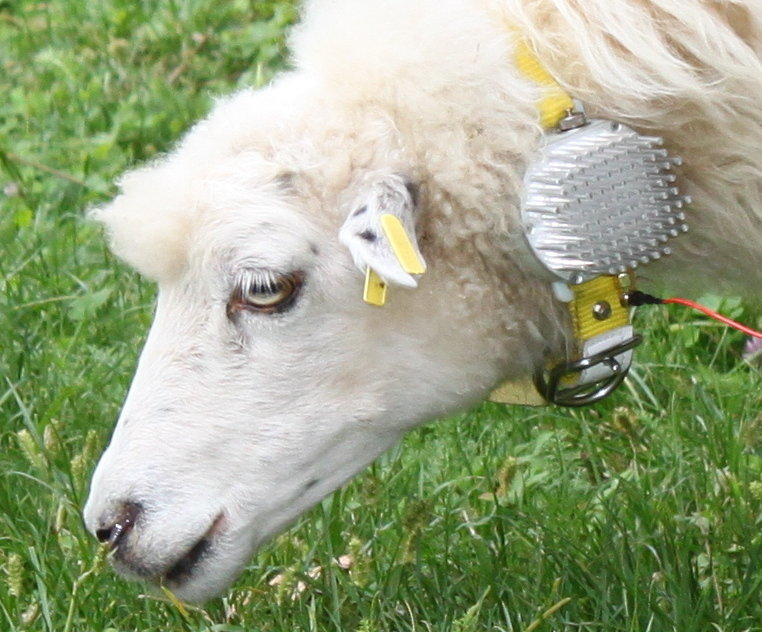
\includegraphics[width=\columnwidth]{img005}
\caption{The device attached to the neck of a sheep with a collar~\cite{baumker2018development}. My proposal idea is to do the same as presented on this image. From here, we can provide algorithms audio information of the individual, as well as the surrounding animals. The animals can be ships, cows, pigs, between others.}
\label{fig:img005}
\end{figure}

\hfill

%%%%%%%%%%%%%%%%%%%%%%%%%%%%%%%%%%%%%%%%%%%%%%%%%%

From PAM data, it presents the challenge of classifying calls from several vocalizing animals of a heard.
This approach is made by moving beyond an animal focus and towards deriving community information.
For most data heterogeneity, this is currently either impossible or extremely difficult, which emphasizes the need for acoustic indicators (Figure \ref{fig:img002}.g).
The acoustic indicators are, therefore, improving the recorded data.
For example, by designating acoustic entropy and dissimilarity indices as acoustic analogs of classical diversity indices~\cite{sueur2008rapid}.

Newer ML methods may offer alternative means to tackle the problem of livestock monitoring.
Looking further, by using Computational Neural Networks (CNN) to quantify and separate sound, we can explicitly bypass the issue of noise sensitive.
Besides, another promising path involves unsupervised learning of acoustic patterns.
Such patterns are directly related to acoustic data.
As an example of this, we can use sparse techniques to isolate periodic sound components within call recording~\cite{underwood2002pain}, which suggest a correlation with animal health issues.